\section{Background}
\label{section:background}
\subsection{Differential Equations}
\subsubsection{Why are Differential Equations important?}
Differential Equations are extremely powerful in their ability to model various systems in applied mathematics, physics, and engineering. Calculus is the mathematics of change. Hence, differential equations, which relate the derivatives or integrals of a function to the function itself, can very elegantly summarize the behavior of otherwise complex, dynamic systems.

For example, the Lotka-Volterra equations describe the dynamics of populations of predators and prey. These equations are described below.

\[\frac{dx}{dt} = \alpha x - \beta x y\]
\[\frac{dy}{dt} = \delta x y - \gamma y\]

\noindent
where:
\begin{itemize}
    \item $x$ is the population density of the prey.
    \item $y$ is the population density of the predator.
    \item $\alpha$ is the exponential growth rate of the prey.
    \item $\gamma$ is the exponential decay rate of the predators.
    \item $\beta$ is the effect of the predators on the prey growth rate.
    \item $\delta$ is the effect of the presence of prey on the predator growth rate.
\end{itemize}

This system is a set of first-order, nonlinear ODEs. This is further explained in Section \ref{subsubsection:properties_differential} \nameref{subsubsection:properties_differential}.

\subsubsection{Properties of Differential Equations}
\label{subsubsection:properties_differential}
\begin{definition}
    The order of a system of differential equations is defined as the highest-order derivative the system contains. Since the highest order derivative in the Lotka-Volterra equations is $\frac{d}{dt}$ (no $\frac{d^2}{{dt}^2}$, the equations are first-order.
\end{definition}

\begin{definition}
    A system of differential equations is said to be linear if and only if the equations follow the form:
    \[ a_0 y + a_1 y' + a_2 y'' \dots + a_n y^{(n)} = b(x) \]
    \noindent
    where $a_0, a_1, a_2, ..., a_n$ are any differentiable functions (do not need to be linear).
\end{definition}

\subsubsection{Solution to Differential Equations}
Note that the solution to a differential equation is not one function, but rather a set of functions that all satisfy the differential equation. Some initial conditions must be given to reduce the solution to a single function. For example, for the Lotka-Volterra equations, the phase space shown in Figure \ref{fig:lotka_volterra_phase} plots the various function solutions given various different initial conditions. The solution for a specific initial condition over time is plotted in Figure \ref{fig:lotka_volterra_init}

\begin{figure}[H]
    \centering
    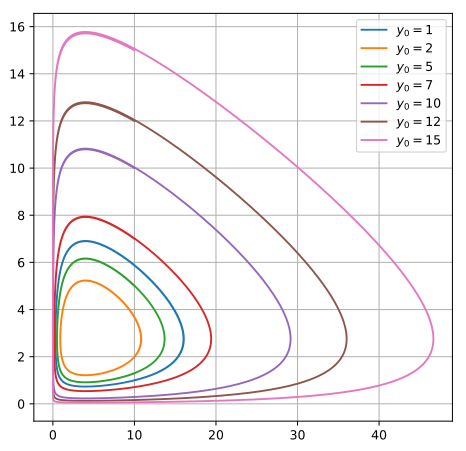
\includegraphics[width=75mm,height=\textheight,keepaspectratio]{images/Predator_prey_dynamics.png}
    \caption{Solution to the Lotka-Volterra Equations given different predator initial conditions. The predator solution is shifted $\frac{\pi}{2}$ radians right of the prey solution.}
    \label{fig:lotka_volterra_phase}
\end{figure}

\begin{figure}[H]
    \centering
    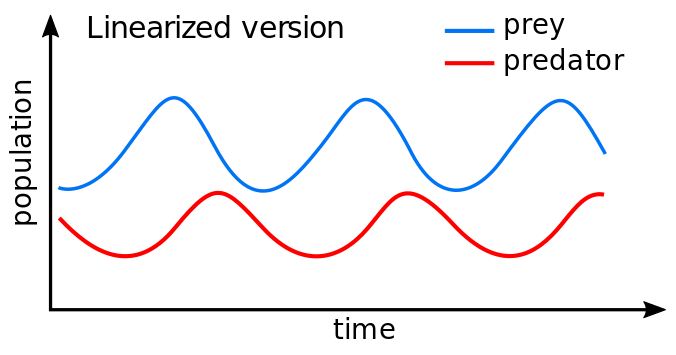
\includegraphics[width=75mm,height=\textheight,keepaspectratio]{images/Lotka_Volterra_dynamics.png}
    \caption{Solution to the Lotka-Volterra Equations given some initial conditions. The predator solution is shifted $\frac{\pi}{2}$ radians right of the prey solution.}
    \label{fig:lotka_volterra_init}
\end{figure}

\subsubsection{ODE vs PDE}
% \lipsum[2]

\subsection{Fourier Analysis}
\subsubsection{What is Fourier Analysis?}
Fourier Analysis is a field of mathematics that studies how complex function waveforms can be decomposed into a series of sinusoidal functions, whose frequencies form a harmonic series. In other words, the Fourier Transform (FT), the cornerstone of Fourier Analysis, turns a signal in time space into a signal in frequency space and a signal in real space into a signal in Fourier space.

\subsubsection{Fourier and Inverse Fourier Transforms}
\begin{definition}
    For a continuous function $f(x)$, the continuous Fourier Transform $\mathcal{F}\{ f(x) \}$ (CFT) is defined as below. The transform returns the frequency space function $\hat{f}(\omega)$.
    \[ \hat{f}(\omega) = \mathcal{F}\{ f(x) \} = \int_{-\infty}^{\infty} f(x)  \, e^{-i 2\pi \omega x} \,dx \]
\end{definition}

%%%%%%%%%%%%%%%%%%%%%%%%%%%%%%%%%%%%%%%%%%%%%%%%%%%%%%%%%%%%%%%%%%%%%%%%%%%%%%%%

\begin{definition}
    In order to reverse the Fourier Transform, the Inverse Fourier Transform $\mathcal{F}^{-1}\{ \hat{f}(\omega) \}$ (IFFT) can be applied as defined below.
    \[ f(x) = \mathcal{F}^{-1}\{ \hat{f}(\omega) \} = \int_{-\infty}^{\infty} \hat{f}(\omega) \, e^{i 2\pi \omega x} \,d \omega \]
\end{definition}

\subsubsection{Fourier Series}
Let \(f(x)\) be defined as the following periodic, yet discontinuous square waveform signal (Heaviside Step Function):

\begin{equation}
f(x)=
    \begin{cases}
        1 & \text{if } nT < x < \frac{T(2n+1)}{2} , n \in \mathbb{Z}\\
        0 & \text{if } x = \frac{nT}{2} , n \in \mathbb{Z}\\
        -1 & \text{if } \frac{T(2n+1)}{2} < x < T(n+1) , n \in \mathbb{Z}
    \end{cases}
\end{equation}

In order to obtain the Fourier Series for \(f(x)\), the Fourier Transform of \(f(x)\) must be taken.

\begin{figure}[H]
    \centering
    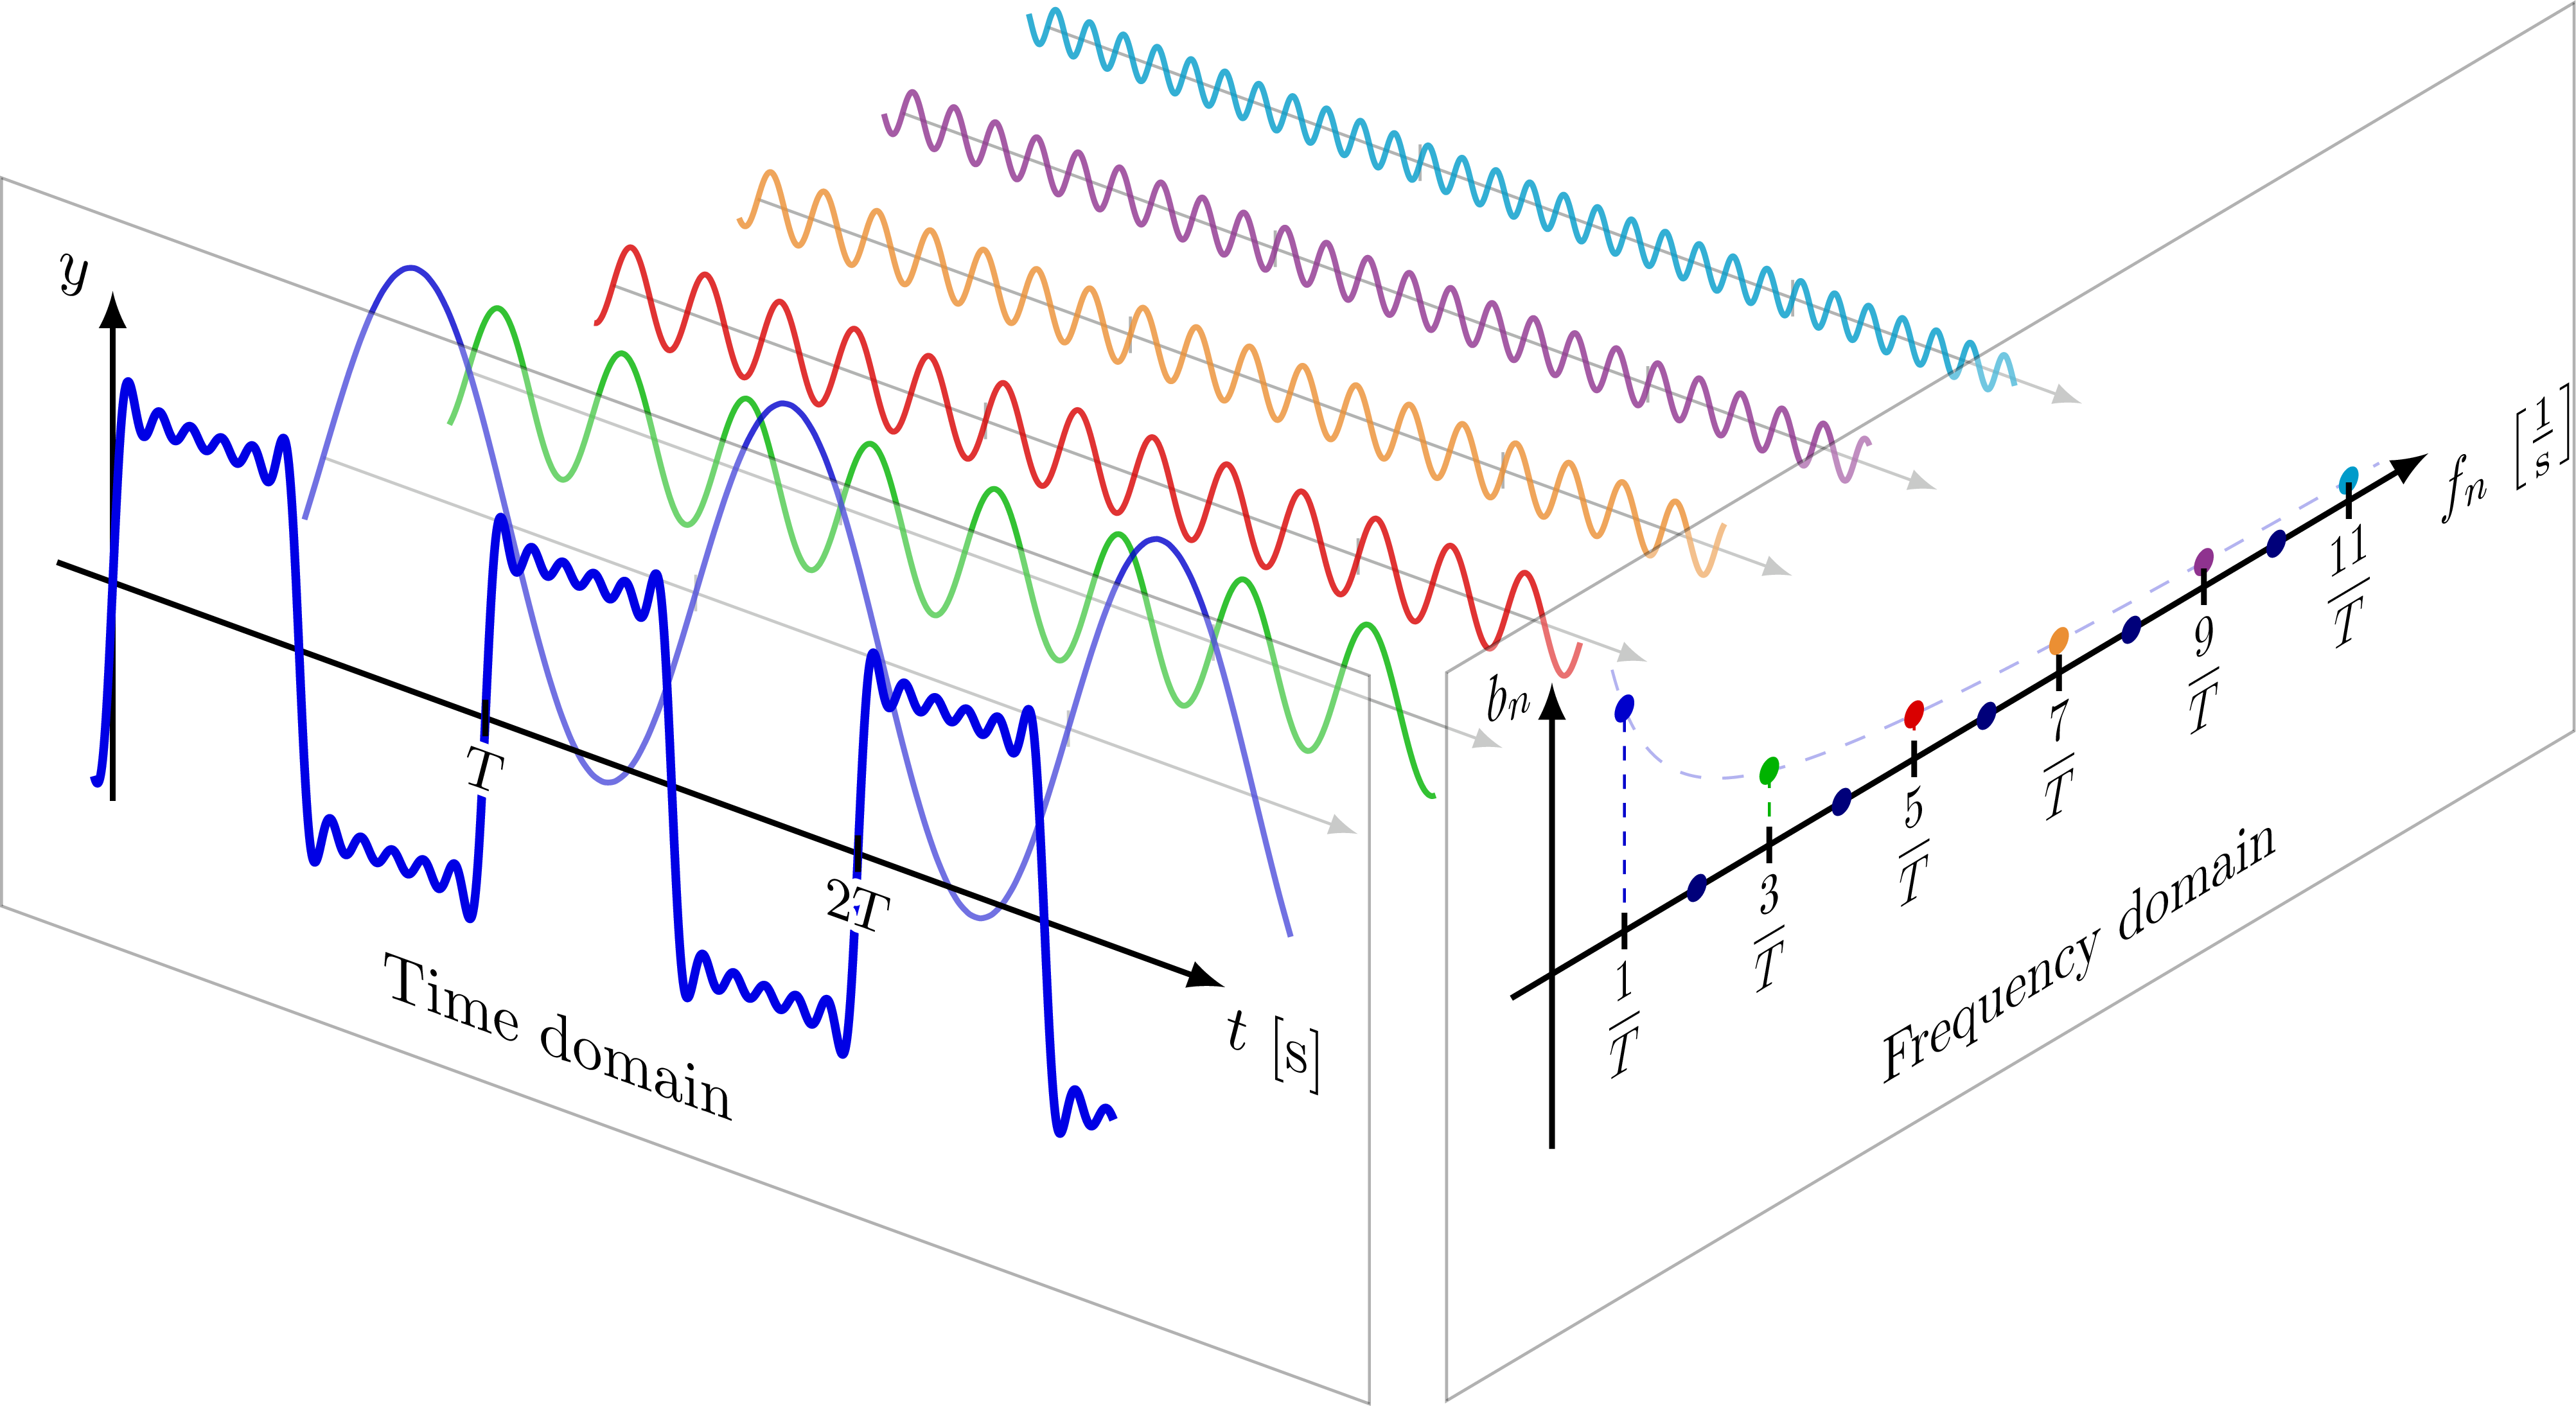
\includegraphics[width=100mm,height=\textheight,keepaspectratio]{images/step_function_fourier_series.png}
    \caption{On the axis to the right, the Fourier Transform of \(f(x)\) can be seen. If an infinite summation of all the frequencies with their corresponding amplitudes was performed as defined by the Fourier Transform, the solution would be exactly equal to \(f(x)\).}
    \label{fig:decomposed_step_function}
\end{figure}

Therefore, f(x) can be defined by the infinite summation of sine functions through its Fourier Series as follows: 
\[f(x)=\frac{4}{\pi}\sum_{n=1,3,5,...}^{\infty} \frac{1}{n} \sin \left( \frac{2 \pi n x}{T}
 \right) \]

\subsubsection{Properties of the Fourier Transform}
The Fourier Transform, which is a coordinate transform, is important and useful because many mathematical operations in Fourier space are simplified compared to the original space. Below are some of the important properties of the Fourier Transform that will be useful in solving differential equations using Fourier Analysis.
\begin{lemma}
    The Fourier Transform is linear. This means that the transform of a linear combination of functions is equal to the linear combination of the transforms of the individual functions.
    \[ \mathcal{F}\{ a f(x) + b g(x) \} = a \mathcal{F}\{ f(x) \} + b \mathcal{F}\{ g(x) \} \]
\end{lemma}
\begin{proof}
    \[ \mathcal{F}\{ a f(x) + b g(x) \} = \int_{-\infty}^{\infty} (a f(x) + b g(x)) \, e^{-i 2\pi \omega x} \,dx \]
    \[ = \int_{-\infty}^{\infty} a f(x) \, e^{-i 2\pi \omega x} \,dx + \int_{-\infty}^{\infty} b g(x) \, e^{-i 2\pi \omega x} \,dx \]
    \[ = a \int_{-\infty}^{\infty} f(x) \, e^{-i 2\pi \omega x} \,dx + b \int_{-\infty}^{\infty} g(x) \, e^{-i 2\pi \omega x} \,dx \]
    \[ = a \mathcal{F}\{ f(x) \} + b \mathcal{F}\{ g(x) \} \]
\end{proof}

%%%%%%%%%%%%%%%%%%%%%%%%%%%%%%%%%%%%%%%%%%%%%%%%%%%%%%%%%%%%%%%%%%%%%%%%%%%%%%%%

\begin{lemma}
    The Fourier Transform can be shifted easily along the axis of the transform. When a function \(f(x)\) along the x-axis by \(x_0\) units, the transform of the shifted function is equal to the transform of the original function multiplied by $e^{-i 2\pi \omega x_0}$.
    \[ \mathcal{F}\{ f(x - x_0) \} = e^{-i 2\pi \omega x_0} \hat{f}(\omega) \]
\end{lemma}

\begin{proof}
    \[ \mathcal{F}\{ f(x - x_0) \} = \int_{-\infty}^{\infty} f(x - x_0) \, e^{-i 2\pi \omega x} \,dx \]
    Let \(u = x - x_0\). Thus, \(x = u + x_0\).
    \[ = \int_{-\infty}^{\infty} f(u) \, e^{-i 2\pi \omega (u + x_0)} \,dx \]
    \[ = e^{-i 2\pi \omega x_0} \int_{-\infty}^{\infty} f(u) \, e^{-i 2\pi \omega u} \,dx \]
    \[ = e^{-i 2\pi \omega x_0} \hat{f}(\omega) \]
\end{proof}

%%%%%%%%%%%%%%%%%%%%%%%%%%%%%%%%%%%%%%%%%%%%%%%%%%%%%%%%%%%%%%%%%%%%%%%%%%%%%%%%
\begin{lemma}
    The Fourier Transform of a function's derivative is equal to the transform of the original function multiplied by $i 2\pi \omega$.
    \[ \mathcal{F}\{ \frac{d f(x)}{dx} \} = i 2\pi \omega \hat{f}(\omega) \]
\end{lemma}

\begin{proof}
    \[ \mathcal{F}\{ \frac{d f(x)}{dx} \} = \int_{-\infty}^{\infty} \frac{d f(x)}{dx}  \, e^{-i 2\pi \omega x} \,dx \]
    Using integration by parts, let \(u = f(x)\) and \(dv = e^{-i 2\pi \omega x} dx\).
    \[ = \left[ f(x) e^{-i 2\pi \omega x} \right]_{-\infty}^{\infty} - \int_{-\infty}^{\infty} f(x) \left( \frac{d}{dx} e^{-i 2\pi \omega x} \right) \,dx \]
    Since \(f(x)\) must be continuous and integrable to be differentiable and take the Fourier Transform on \(\mathbb{R}\), \(\lim_{x \to -\infty}=\lim_{x \to \infty}=0\) must be true. Thus, the first term is equal to zero. 
    \[ = - \int_{-\infty}^{\infty} f(x) \left( -i 2\pi \omega e^{-i 2\pi \omega x} \right) \,dx \]
    \[ = i 2\pi \omega \int_{-\infty}^{\infty} f(x) e^{-i 2\pi \omega x} \,dx \]
    \[ = i 2\pi \omega \hat{f}(\omega) \]
\end{proof}